\documentclass[12pt]{article}

\usepackage[utf8]{inputenc}
\usepackage{latexsym,amsfonts,amssymb,amsthm,amsmath,graphicx,mathtools,subfig,hyperref}
\usepackage[parfill]{parskip}
\usepackage[export]{adjustbox}
\usepackage[justification=centering]{caption}
\usepackage{nameref}

\hypersetup{
    colorlinks=true,
    linkcolor=blue,
    filecolor=magenta,      
    urlcolor=cyan,
}

\DeclareMathAlphabet{\mymathbb}{U}{BOONDOX-ds}{m}{n}

\setlength{\parindent}{0in}
\setlength{\oddsidemargin}{0in}
\setlength{\textwidth}{17cm}
\setlength{\textheight}{22cm}
\setlength{\topmargin}{0cm}
\setlength{\headheight}{0pt}
\setlength{\footskip}{30pt}

\DeclareMathOperator*{\argmax}{arg\,max}
\DeclareMathOperator*{\argmin}{arg\,min}

\newcommand{\expax}{e^{\mathbf{a}_{i}^T\mathbf{x}_{b_{i}}}}
\newcommand{\expaxj}{e^{\mathbf{a}_{i}^T\mathbf{x}_j}}
\newcommand{\expaxsum}{\sum_{k=1}^{C} e^{\mathbf{a}_{i}^T\mathbf{x}_k}}
\newcommand{\boldX}{\mathbf{X}}
\newcommand{\aat}{\mathbf{a}_{i} \mathbf{a}_{i}^{T}}
\newcommand{\bigsigma}{\mathbf{\Sigma}_{i}}

\title{EE-556 Homework 3}
\author{Edoardo Debenedetti}

\begin{document}

\maketitle

\section{Multiclass classification}

\subsection{Theory}

\subsubsection{Multinomial logistic regression estimator}
\begin{proof}
Assuming that we can write $\mathbb{P}(b_{i} = j | \mathbf{a}_{i}, \mathbf{X})$ as
\begin{equation}
    \mathbb{P}(b_{i} = j | \mathbf{a}_{i}, \mathbf{X}) = \frac{\expaxj}{\expaxsum}
\end{equation}

And that all the samples in the matrix $\mathbf{A}$ are i.i.d., we can write $\mathbb{P}(\mathbf{b} | \mathbf{A}, \mathbf{X})$ as
\begin{equation}
    \mathbb{P}(\mathbf{b} | \mathbf{A}, \mathbf{X}) = \prod_{i=1}^n \frac{\expax}{\expaxsum}
\end{equation}

Then, we can write $\hat{\boldX}_{ML}$ as
\begin{equation}
    \hat{\boldX}_{ML} \in \argmax_{\boldX} \left \{ \prod_{i=1}^n \frac{\expax}{\expaxsum} \right\}
\end{equation}

However, as we are interested in taking the $\argmax_{\boldX}$, we can take the logarithm of the argument, since $\log$ is strictly increasing and does not change the $\argmax_{\boldX}$:
\begin{gather}
    \argmax_{\boldX} \left \{ \prod_{i=1}^n \frac{\expax}{\expaxsum} \right\}
    = \argmax_{\boldX} \left \{ \log \prod_{i=1}^n \frac{\expax}{\expaxsum} \right\} = \label{eq:x-ml-first} \\
    = \argmax_{\boldX} \left \{ \sum_{i=1}^n \log \frac{\expax}{\expaxsum} \right\} = \label{eq:x-ml-second} \\
    = \argmax_{\boldX} \left \{ \sum_{i=1}^n \left ( \log \expax - \log \expaxsum \right ) \right\} = \label{eq:x-ml-third} \\
    = \argmax_{\boldX} \left \{ \sum_{i=1}^n \left ( \mathbf{a}_{i}^T\mathbf{x}_{b_{i}} - \log \expaxsum \right ) \right\}
\end{gather}

Between \eqref{eq:x-ml-first} and \eqref{eq:x-ml-second} we exploited the fact that the log of the products is equal to the sum of the logs, and between \eqref{eq:x-ml-second} and \eqref{eq:x-ml-third} we exploited the fact that the log of a ratio is the difference of the logs. We can now take the negative of the argument of $\argmax_{\boldX}$ and transform $\argmax_{\boldX}$ in $\argmin_{\boldX}$:
\begin{gather}
    \argmax_{\boldX} \left \{ \sum_{i=1}^n \left ( \mathbf{a}_{i}^T\mathbf{x}_{b_{i}} - \log \expaxsum \right ) \right\} = \\
    = \argmin_{\boldX} \left \{ \sum_{i=1}^n \left (\log \expaxsum - \mathbf{a}_{i}^T\mathbf{x}_{b_{i}} \right ) \right\}
\end{gather}

Hence:
\begin{equation} \label{eq:ml-estmator}
    \hat{\boldX}_{ML} \in \argmin \left \{ f(\boldX) | f: \mathbb{R}^{d \times C} \rightarrow \mathbb{R}, f(\boldX) = \sum_{i=1}^n \left (\log \expaxsum - \mathbf{a}_{i}^T\mathbf{x}_{b_{i}} \right ), b_{i} \in \{1, 2, ... C\} \right \}
\end{equation}

Which is the form for $\hat{\boldX}_{ML}$ we had to prove.
\end{proof}

\subsubsection{Multinomial logistic regression estimator gradient}
\begin{proof}
Since both sum and subtraction are linear, we can re-write $f(x)$ defined in \eqref{eq:ml-estmator} as
\begin{equation}
    f(\boldX) = \sum_{i=1}^n \log \expaxsum - \sum_{i=1}^n \mathbf{a}_{i}^T\mathbf{x}_{b_{i}}
\end{equation}

First, let us take in consideration the left part of $f(\boldX)$: 

\end{proof}


\stepcounter{subsubsection}
\subsubsection{Lipschitz constant}

\paragraph{(a) Maximum eigenvalue \texorpdfstring{$\lambda_{max}(\aat)$}{Lg}} \label{par:max-eig}
\begin{proof}
Given $\mathbf{a}_i \in \mathbb{R}^{n}$, as $\aat$ is rank-1, $n-1$ eigenvalues of $\aat$ are $0$, and only 1 is non-zero. This means that, as the sum of the eigenvalues of a matrix is given by its trace,
\begin{equation} \label{eq:maxeig-tr}
    \lambda_{max}(\aat) = Tr(\aat)
\end{equation}

Moreover, since $\aat$ is the matrix whose $k,l$-th element is given by $a_{i,k}a_{i,l}$, its $k$-th diagonal element is given by $a_{i,k}a_{i,k} = a_{i,k}^{2}$, and then
\begin{equation} \label{eq:tr-2norm}
    Tr(\aat) = \sum_{k=1}^{n} a_{i,k}^{2} = \lVert \mathbf{a}_{i} \rVert ^{2}
\end{equation}

Finally, combining \eqref{eq:maxeig-tr} and \eqref{eq:tr-2norm}, we get
\begin{equation}
    \lambda_{max}(\aat) = \lVert \mathbf{a}_{i} \rVert ^{2}
\end{equation}

\end{proof}

\paragraph{(b) Lipschitz constant of the gradient}
\begin{proof}
Given $\nabla^f(\boldX) = \sum_{i=1}^{n} \bigsigma \otimes \aat$ and the fact that we can choose $L = \frac{\lVert A \rVert_{F}^{2}}{2}$ if
\begin{equation} \label{eq:L-condition}
    \lambda_{max}(\nabla^{2}f(\boldX)) \leq \frac{\lVert A \rVert_{F}^{2}}{2} < \infty
\end{equation}

We should then look for an upper-bound for $\lambda_{max}(\nabla^{2}f(\boldX))$. We proved that $\lambda_{max}(\aat) = \lVert \mathbf{a}_{i} \rVert ^{2}$. Now, let us look for the maximum eigenvalue of $\bigsigma$. We also know from exercise 1.1.2 that both $\bigsigma \succeq 0$ and $\aat \succeq 0$, $\forall i \in [1, n]$. Then, as $\bigsigma \succeq 0$, its $\lambda_{max}(\bigsigma) \leq \max_{k} \sum_{l} |\mathbf{\Sigma}_{i,kl}|$. If them we take the $\ell$-1 norm of each row of $\bigsigma$, we get
\begin{equation} \label{eq:sigma-onenorm}
\lVert \bigsigma{}_{j} \rVert_{1} = |\sigma_{ij}(1 - \sigma_{ij})| + \sum_{k=1,k \neq j}^{C} | -\sigma_{ij}\sigma_{ik}| 
\end{equation}

Moreover, as each $\sigma$ is a probability, $0 \leq \sigma_{ij} \leq 1, \forall i,j$. Then:
\begin{itemize}
    \item The product between two $\sigma$ is positive
    \item $1 - \sigma_{ij} \geq 0, \forall i,j$
\end{itemize}
Then we can remove the absolute values and the minus inside the sum from \eqref{eq:sigma-onenorm} and rewrite it as
\begin{equation} \label{eq:sigma-onenorm-2}
    \lVert \bigsigma{}_{j} \rVert_{1} = \sigma_{ij}(1 - \sigma_{ij}) + \sigma_{ij} \sum_{k=1,k \neq j}^{C} \sigma_{ik}
\end{equation}

It is worth noting that $\sigma_{ij}$ has been taken outside the sum as it does not depend on $k$. Moreover, we can write $\sum_{k=1,k \neq j}^{C} \sigma_{ik}$ as $1 - \sigma_{ij}$. Then \eqref{eq:sigma-onenorm-2} becomes
\begin{gather} \label{eq:sigma-onenorm-3}
    \lVert \bigsigma{}_{j} \rVert_{1} = \sigma_{ij}(1 - \sigma_{ij}) + \sigma_{ij}(1 - \sigma_{ij}) = 2 \sigma_{ij}(1 - \sigma_{ij}) = 2(\sigma_{ij} - \sigma_{ij}^{2})
\end{gather}

We are now interested in the maximum $\lVert \bigsigma{}_{j} \rVert_{1}$ possible. Since $\sigma_{ij}$ is concave, and so is $-\sigma_{ij}^{2}$, and since $\sigma_{ij} + (-\sigma_{ij}^{2})$ is the sum of two concave functions, it is concave as well. We can then look for a local maximum that will be also a global one. We can than take the derivative of $ \lVert \bigsigma{}_{j} \rVert_{1}$ as a function of $\sigma_{ij}$ to 0 and look for the maximizing $\sigma_{ij}$:
\begin{equation}
    \frac{\mathrm{d}}{\mathrm{d}\sigma_{ij}}(\sigma_{ij} - \sigma_{ij}^{2}) =  1 - 2 \sigma{ij}
\end{equation}

Setting the derivative to 0 gives us
\begin{equation}
    \sigma_{ij} = \frac{1}{2}
\end{equation}

Plugging it into \eqref{eq:sigma-onenorm-3} we obtain
\begin{equation}
    2(\sigma_{ij} - \sigma_{ij}^{2}) | _{\sigma_{ij} = \frac{1}{2}} = \frac{1}{2}
\end{equation}

Then we get that
\begin{equation}
    \lambda_{max}(\bigsigma) \leq \max_{k} \sum_{l} |\mathbf{\Sigma}_{i,kl}| \leq \frac{1}{2}
\end{equation}

Hence,
\begin{equation}
    \lambda_{max}(\bigsigma) \leq \frac{1}{2}
\end{equation}

Recalling that both $\bigsigma \succeq 0$ and $\aat \succeq 0$, $\forall i \in [1, n]$, then
\begin{equation}
    \lambda_{max}(\bigsigma \otimes \aat) = \lambda_{max}(\bigsigma) \lambda_{max}(\aat)
\end{equation}

Using the upper-bounds we have found above, we can then state that
\begin{equation}
    \lambda_{max}(\bigsigma \otimes \aat) = \frac{1}{2} \lVert \mathbf{a}_i \rVert_{2}^{2}
\end{equation}

Moreover, $\bigsigma$ is symmetric by construction, and as it has only real entries, it is Hermitian. Due to the structure described above, also $\aat$ is symmetric and real, then it is Hermitian. Moreover, since $A^T \otimes B^T = (A \otimes B)^T$, if $A = A^T$ and $B = B^T$, then $(A \otimes B) = (A^T \otimes B^T) = (A \otimes B)^T$. Then, in the specific case where $A = \bigsigma$ and $B = \aat$, $(\bigsigma \otimes \aat) = (\bigsigma \otimes \aat)^T$. As also $\bigsigma \otimes \aat$ has only real entries, it is Hermitian.

Finally, because of Weyl's inequality, we know that $\lambda_{max}(A + B) \leq \lambda_{max}(A) + \lambda_{max}(B)$ if $A$ and $B$ are both Hermitian. Then,
\begin{equation}
    \lambda_{max} \left (\sum_{i=1}^{n} \bigsigma \otimes \aat \right) \leq \sum_{i=1}^{n} \lambda_{max} (\bigsigma \otimes \aat) \leq \sum_{i=1}^{n} \frac{1}{2} \lVert \mathbf{a}_i \rVert_{2}^{2} = \frac{\lVert \mathbf{A} \rVert_{F}^{2}}{2}
\end{equation}

That is what we were looking for in \eqref{eq:L-condition}.
\end{proof}

\subsubsection{\texorpdfstring{$\ell$}{Lg}-1 Proximal operator}
\begin{proof}
Given $g(\mathbf{x}) := \lVert \mathbf{x} \rVert_1$,
\begin{equation}
    prox_{\lambda g}(\mathbf{z}) = \argmin_{\mathbf{y}} \{\lambda \lVert \mathbf{y} \rVert_1 + \frac{1}{2} \lVert \mathbf{y} - \mathbf{z} \rVert_2^2 \}
\end{equation}

As both the functions inside the $\argmin$ are convex with respect to $\mathbf{y}$, sum is convex. We can then find the minimizer $\mathbf{y}_{min}$ by taking its gradient with respect to $\mathbf{y}$ to 0.

If we assume $z \in \mathbb{R}$ also $y \in \mathbb{R}$, the argument of $\argmin$ becomes $\lambda |y| + \frac{1}{2} (y - z)^2$ and we can find the derivative with respect to $y$:
\begin{gather}
     \frac{\mathrm{d}}{\mathrm{dy}} [\lambda |y| + \frac{1}{2} (y - z)^2] = \\
     = \lambda sign(y) + y - z = \\
     = \begin{cases}
     - \lambda + y - z, & y < 0 \\
     \lambda + y - z, & y > 0
     \end{cases}
\end{gather}

Equating it to zero, we obtain:
\begin{equation} \label{y-min-nosubgr}
     y_{min} = \begin{cases}
     \lambda + z, & y < 0, z < -\lambda \\
     z - \lambda, & y > 0, z > \lambda
     \end{cases}
\end{equation}

We can see that $y_{min}$ is only defined in the zone where $|z| > \lambda$ (since $\lambda > 0$), as $|y|$ is not differentiable in $y = 0$, and then its derivative is not defined there. However, in order to find the prox operator, we can also use the subdifferential, and we can choose as subgradient $0$ and then \eqref{y-min-nosubgr} becomes
\begin{equation} \label{y-min-subgr}
     y_{min} = \begin{cases}
     \lambda + z,   & z < -\lambda \\
     z - \lambda,   & z > \lambda \\
     0,             & |z| < \lambda 
     \end{cases}
\end{equation}

However, we can rewrite \eqref{y-min-subgr} as
\begin{equation} \label{y-min-penultimate}
     y_{min} = \begin{cases}
     \max (z - \lambda, 0),   & z \geq 0 \\
     \max (-z - \lambda, 0),   & z < 0
     \end{cases}
\end{equation}

Which can be compressed into the form
\begin{equation}
    y_{min} = \max(|z| - \lambda, 0) \cdot sign(z)
\end{equation}

Since $\lambda \lVert \mathbf{y} \rVert_1 + \frac{1}{2} \lVert \mathbf{y} - \mathbf{z} \rVert_2^2 = \sum_{i=1}^{d}|y_i| + \frac{1}{2}(y_i - z_i)^2$, each $y_{i, min}$ is given by $y_{y, min} = \max(|z_i| - \lambda, 0) \cdot sign(z_i)$ and we can then the vector $\mathbf{y}$ by applying the operators coordinate-wise, which results in
\begin{equation}
    \mathbf{y}_{min} = \max(|\mathbf{z}| - \lambda, 0) \odot sign(\mathbf{z})
\end{equation}

Finally,
\begin{equation}
    prox_{\lambda g}(\mathbf{z}) = \mathbf{y}_{min} = \max(|\mathbf{z}| - \lambda, 0) \odot sign(\mathbf{z})
\end{equation}

\end{proof}

\subsubsection{\texorpdfstring{$\ell$}{Lg}-2 Proximal operator}
\begin{proof}
Given $g(\mathbf{x}) := \frac{1}{2} \lVert \mathbf{x} \rVert_{2}^{2}$,
\begin{equation}
    prox_{\lambda g}(\mathbf{z}) = \argmin_{\mathbf{y}} \{\frac{\lambda}{2} \lVert \mathbf{y} \rVert_2^2 + \frac{1}{2} \lVert \mathbf{y} - \mathbf{z} \rVert_2^2 \}
\end{equation}

As, again, both the functions inside the $\argmin$ are convex with respect to $\mathbf{y}$, their sum is convex. We can then find the minimizer $\mathbf{y}_{min}$ by taking its gradient with respect to $\mathbf{y}$ to 0:
\begin{equation}
    \nabla \{\frac{\lambda}{2} \lVert \mathbf{y} \rVert_2^2 + \frac{1}{2} \lVert \mathbf{y} - \mathbf{z} \rVert_2^2 \} = \lambda \mathbf{y} + \mathbf{y} - \mathbf{z} = \mathbf{y}(1 + \lambda) - \mathbf{z}
\end{equation}

Taking it to zero we get
\begin{gather}
    \mathbf{y}_{min}(1 + \lambda) = \mathbf{z} \\
    \mathbf{y}_{min} = \frac{\mathbf{z}}{1 + \lambda}
\end{gather}

Which leads to
\begin{equation}
    prox_{\lambda g}(\mathbf{z}) = \frac{\mathbf{z}}{1 + \lambda}
\end{equation}
\end{proof}

\subsection{Handwritten digit classification}

\stepcounter{subsubsection}
\subsubsection{Algorithms implementation and convergence}

\begin{figure}
    \centering
    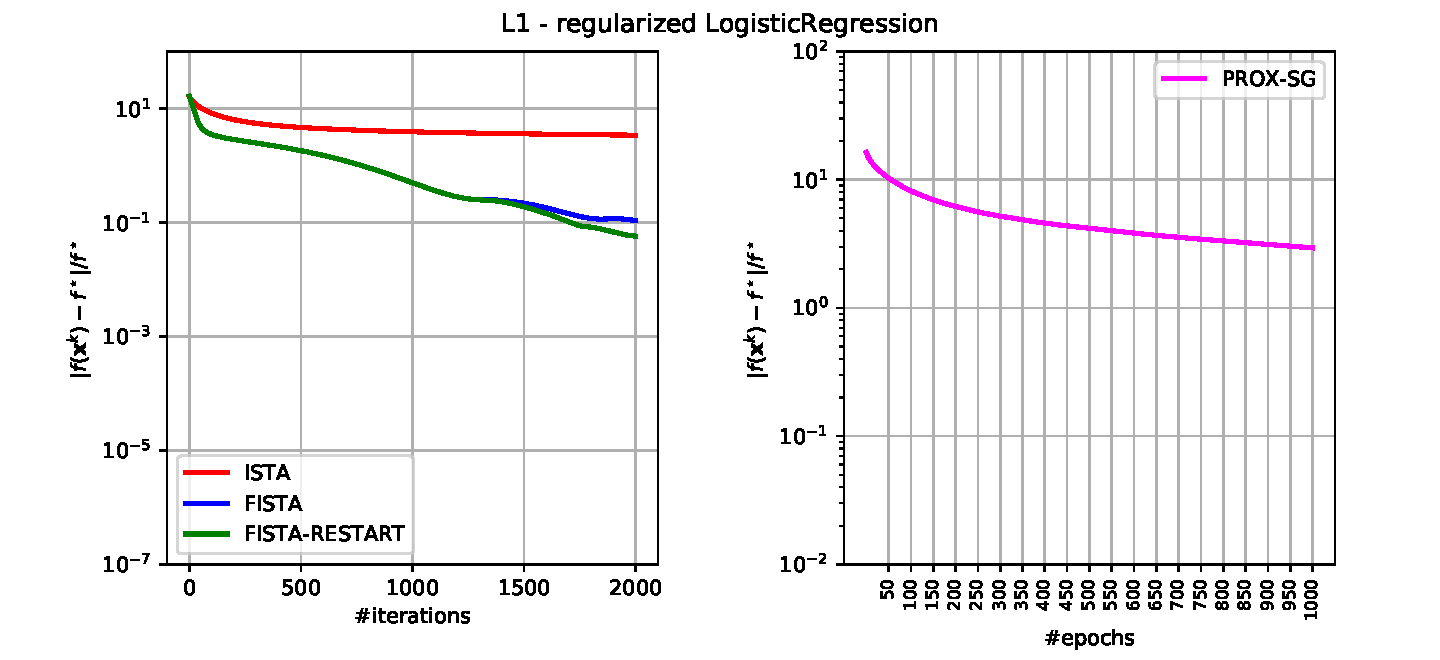
\includegraphics[width=17cm]{hw3/codes/exercise1/results/l1.pdf}
    \caption{Convergence of $\ell$-1 regularized Logistic Regression}
    \label{fig:l1-convergence}
\end{figure}

\begin{figure}
    \centering
    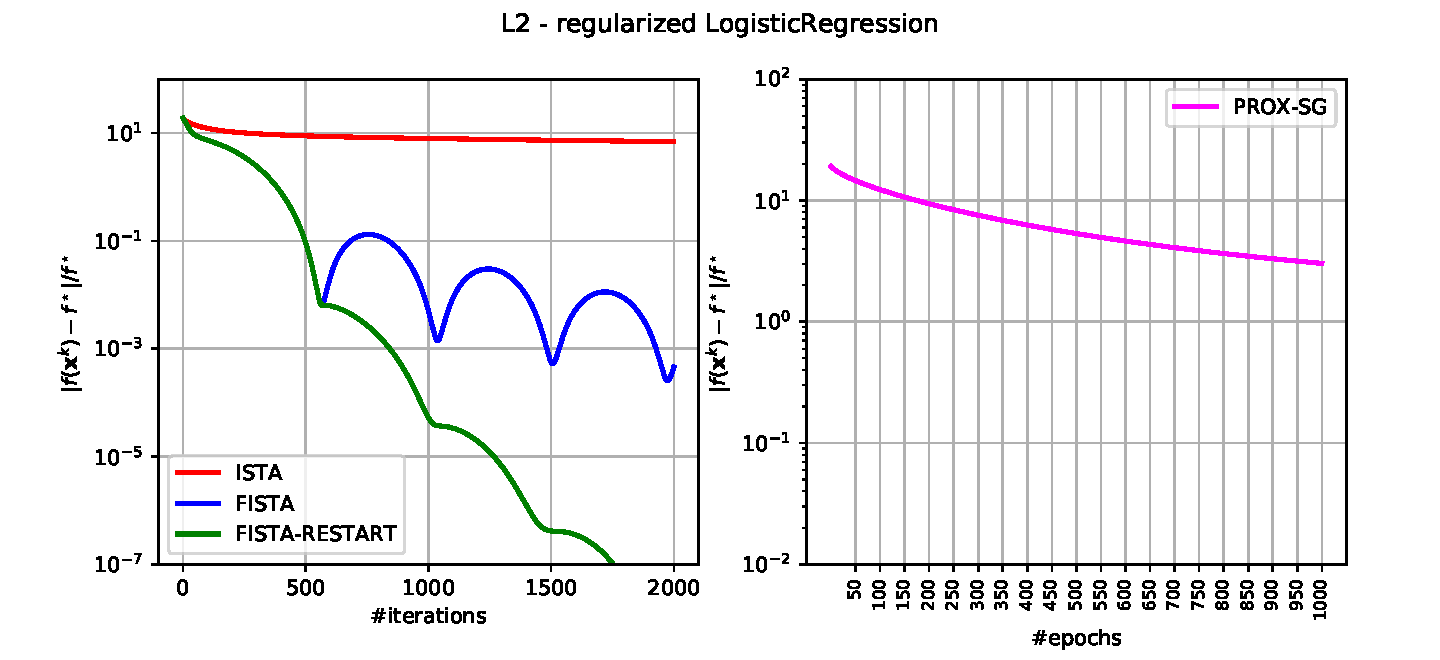
\includegraphics[width=17cm]{hw3/codes/exercise1/results/l2.pdf}
    \caption{Convergence of $\ell$-2 regularized Logistic Regression}
    \label{fig:l2-convergence}
\end{figure}

\begin{figure}
    \centering
    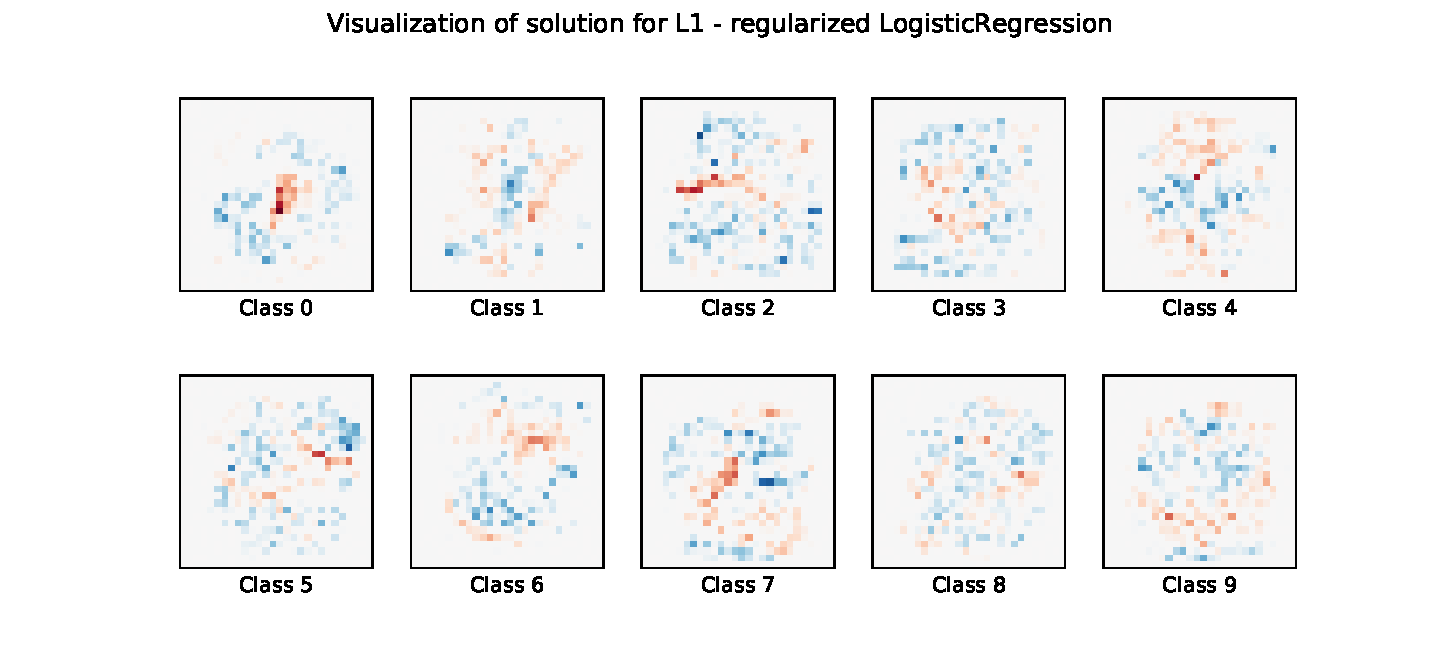
\includegraphics[width=17cm]{hw3/codes/exercise1/results/l1-numbers.pdf}
    \caption{Solution of $\ell$-1 regularized Logistic Regression}
    \label{fig:l1-solution}
\end{figure}

\begin{figure}
    \centering
    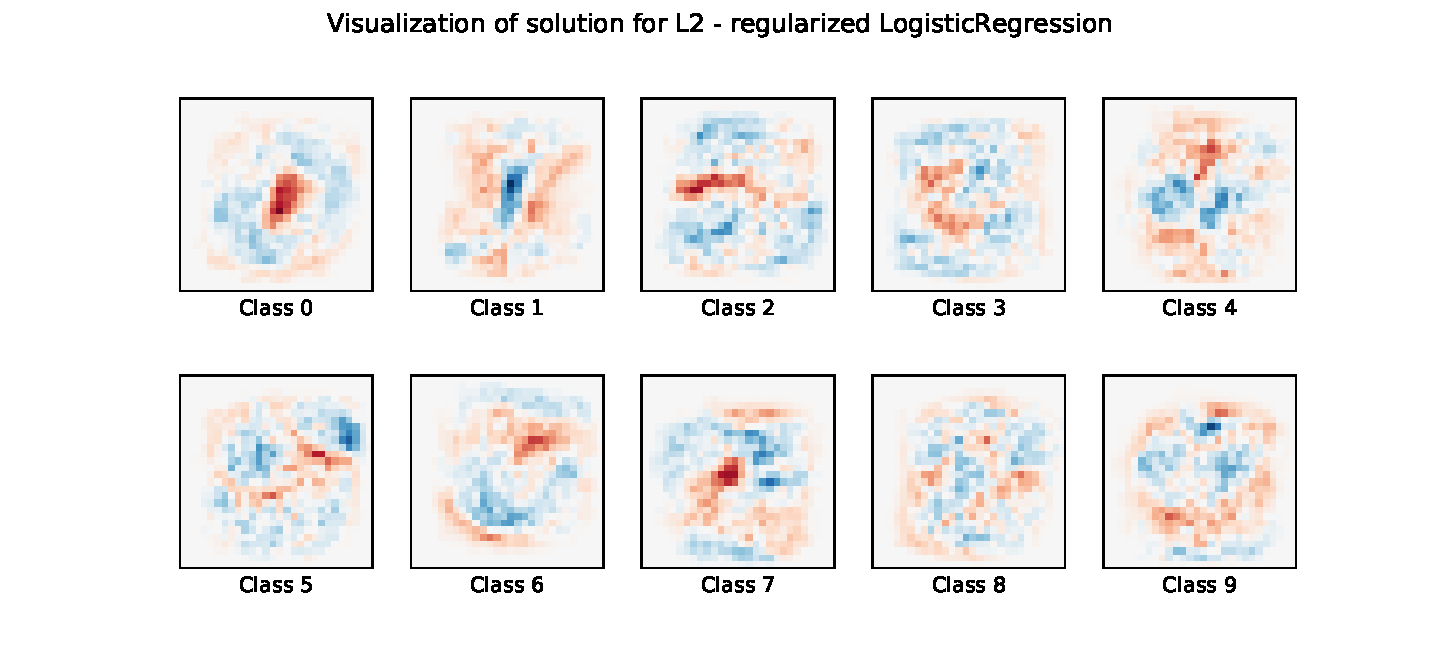
\includegraphics[width=17cm]{hw3/codes/exercise1/results/l2-numbers.pdf}
    \caption{Solution of $\ell$-2 regularized Logistic Regression}
    \label{fig:l2-solution}
\end{figure}

\subsubsection{Logistic Regression and Neural Network comparison}
\begin{itemize}
    \item $\ell$-1 final accuracy = 89.21\%
    \item $\ell$-2 final accuracy = 89.89\%
    \item NN final accuracy = 94.7\%
\end{itemize}

\section{Image reconstruction}
\subsection{Properties of TV and \texorpdfstring{$\ell$}{Lg}-1 in-painting}
\subsubsection{Gradients of TV and \texorpdfstring{$\ell$}{Lg}-1 in-painting}

\subsubsection{Lipschitz constants of TV and \texorpdfstring{$\ell$}{Lg}-1 in-painting}

\subsection{FISTA implementation and \texorpdfstring{$\lambda$}{Lg} sweep}

\begin{itemize}
    \item Best l1 lambda = 0.0013894954943731374
    \item Best tv lambda = 0.0005179474679231213
\end{itemize}{}

\begin{figure}
    \centering
    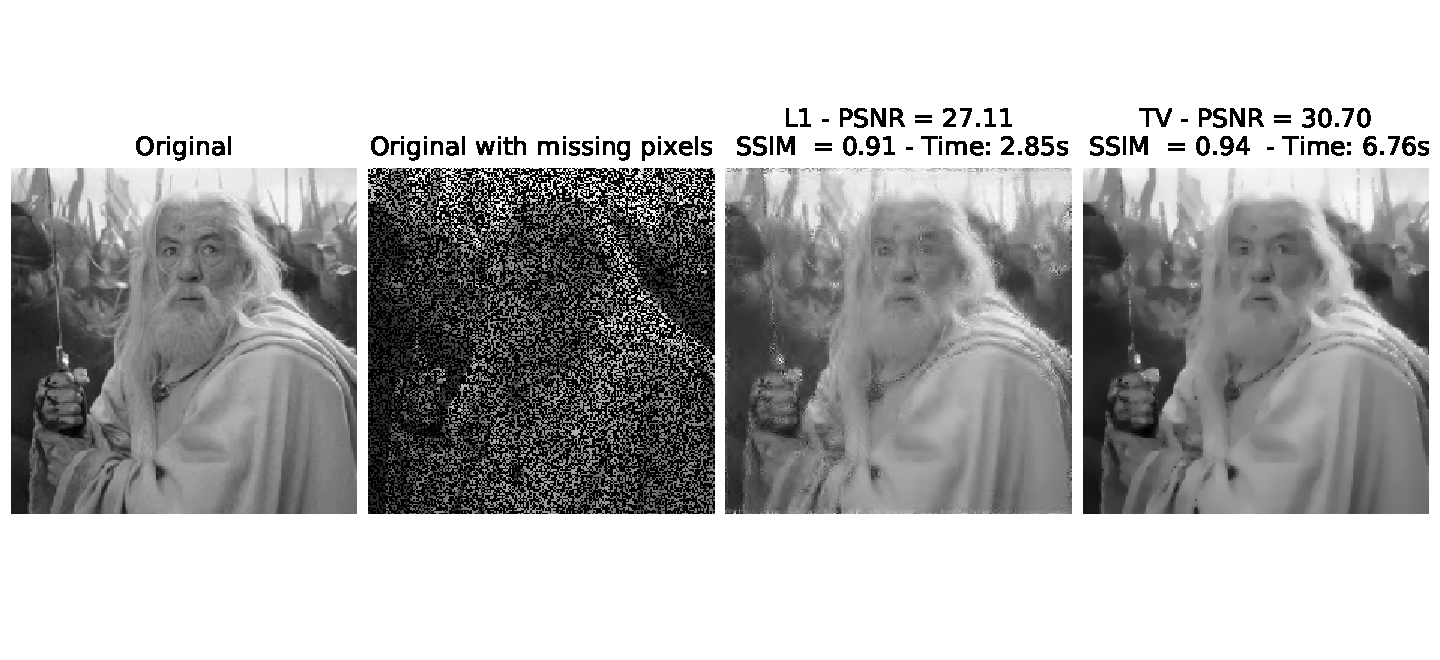
\includegraphics[width=17cm]{hw3/codes/exercise2/results/gandalf_0-01.pdf}
    \caption{Results obtained with $\lambda = 0.01$ on the reference image}
    \label{fig:gandalf-reconstruction}
\end{figure}

\begin{figure}
    \centering
    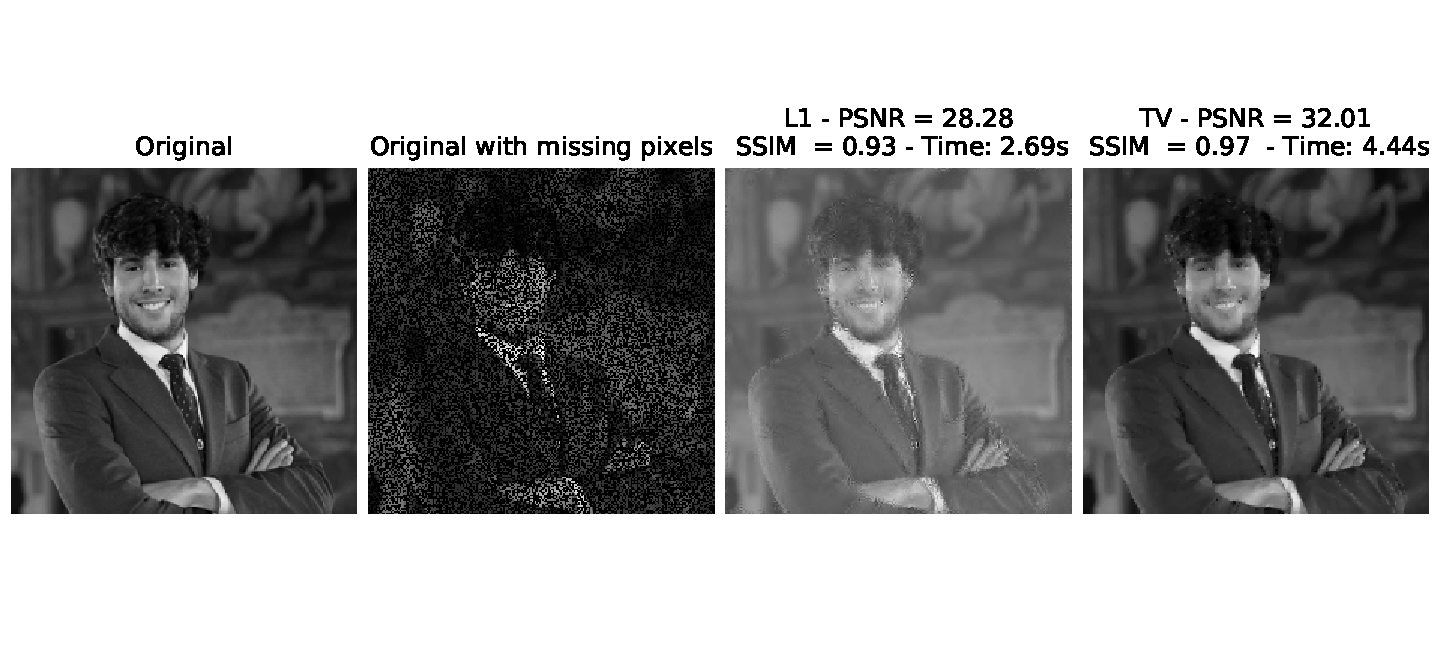
\includegraphics[width=17cm]{hw3/codes/exercise2/results/lambda_search/me_0-001.pdf}
    \caption{Results obtained with $\lambda = 0.001$}
    \label{fig:lambda-search-0.001}
\end{figure}

\begin{figure}
    \centering
    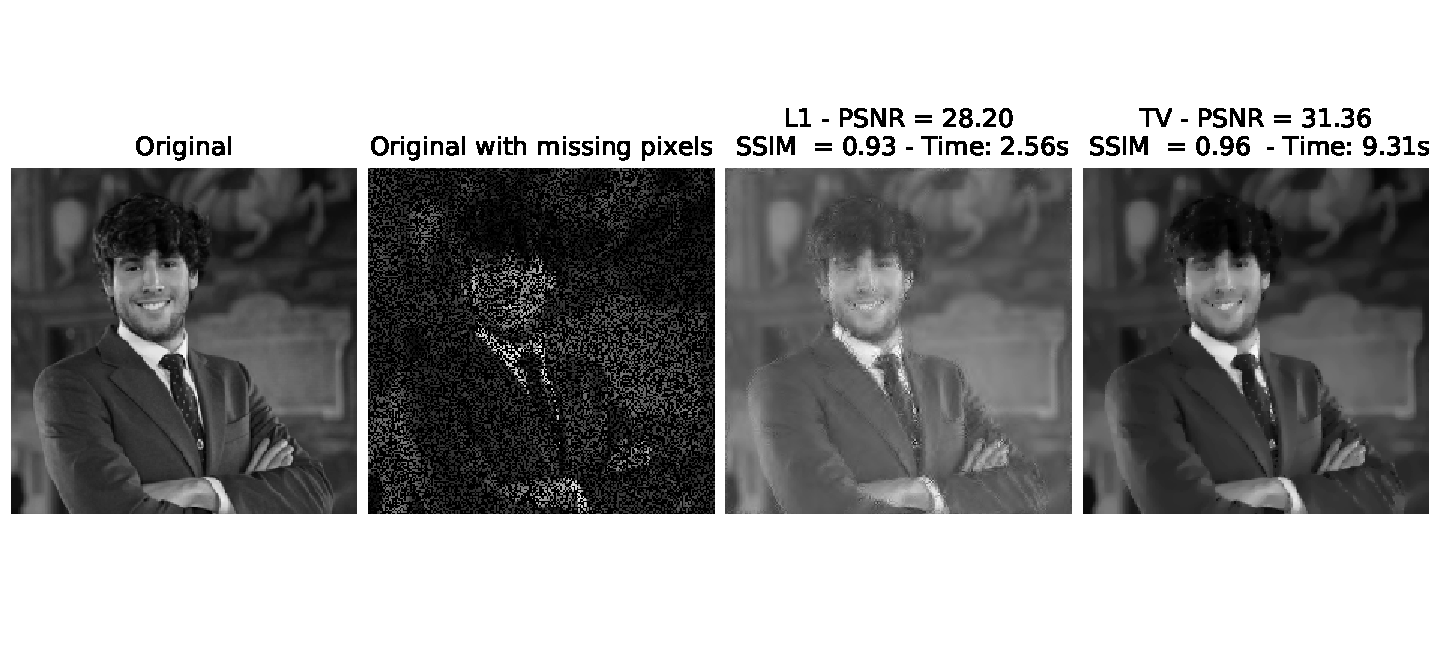
\includegraphics[width=17cm]{hw3/codes/exercise2/results/lambda_search/me_0-01.pdf}
    \caption{Results obtained with $\lambda = 0.01$}
    \label{fig:lambda-search-0.01}
\end{figure}

\begin{figure}
    \centering
    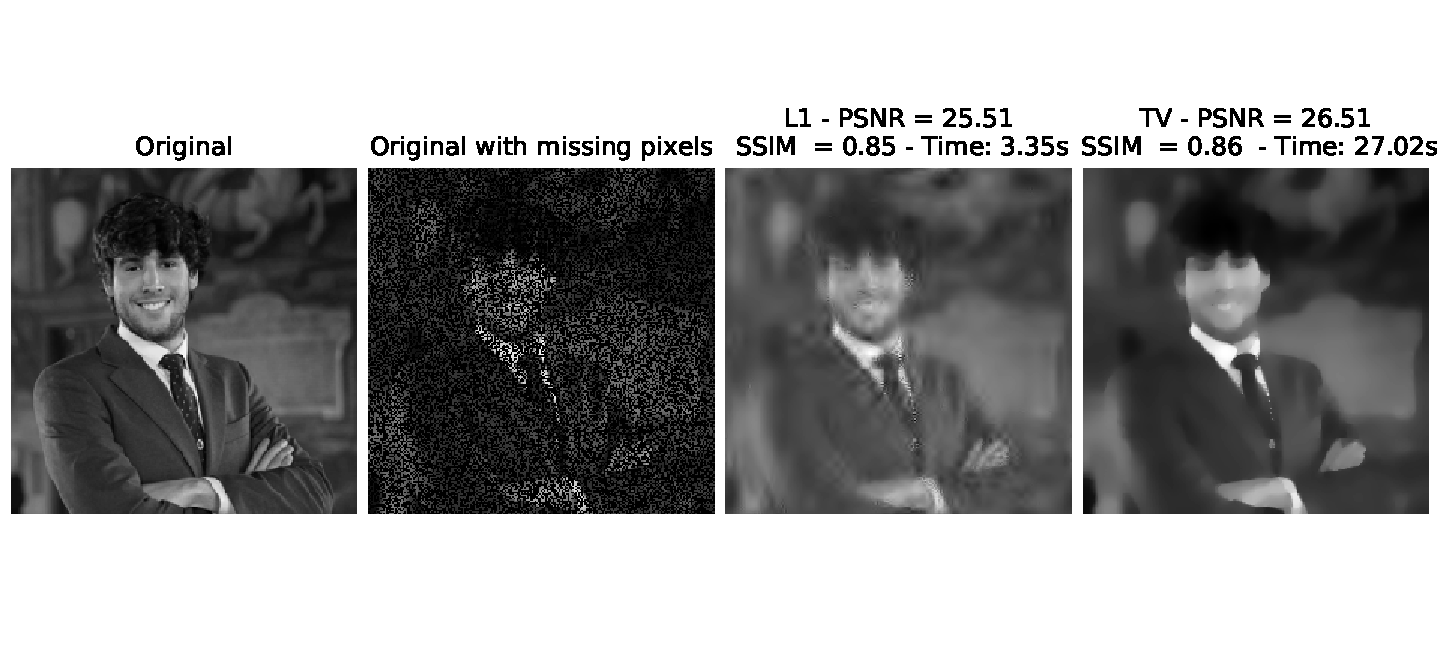
\includegraphics[width=17cm]{hw3/codes/exercise2/results/lambda_search/me_0-1.pdf}
    \caption{Results obtained with $\lambda = 0.1$}
    \label{fig:lambda-search-0.1}
\end{figure}

\begin{figure}
    \centering
    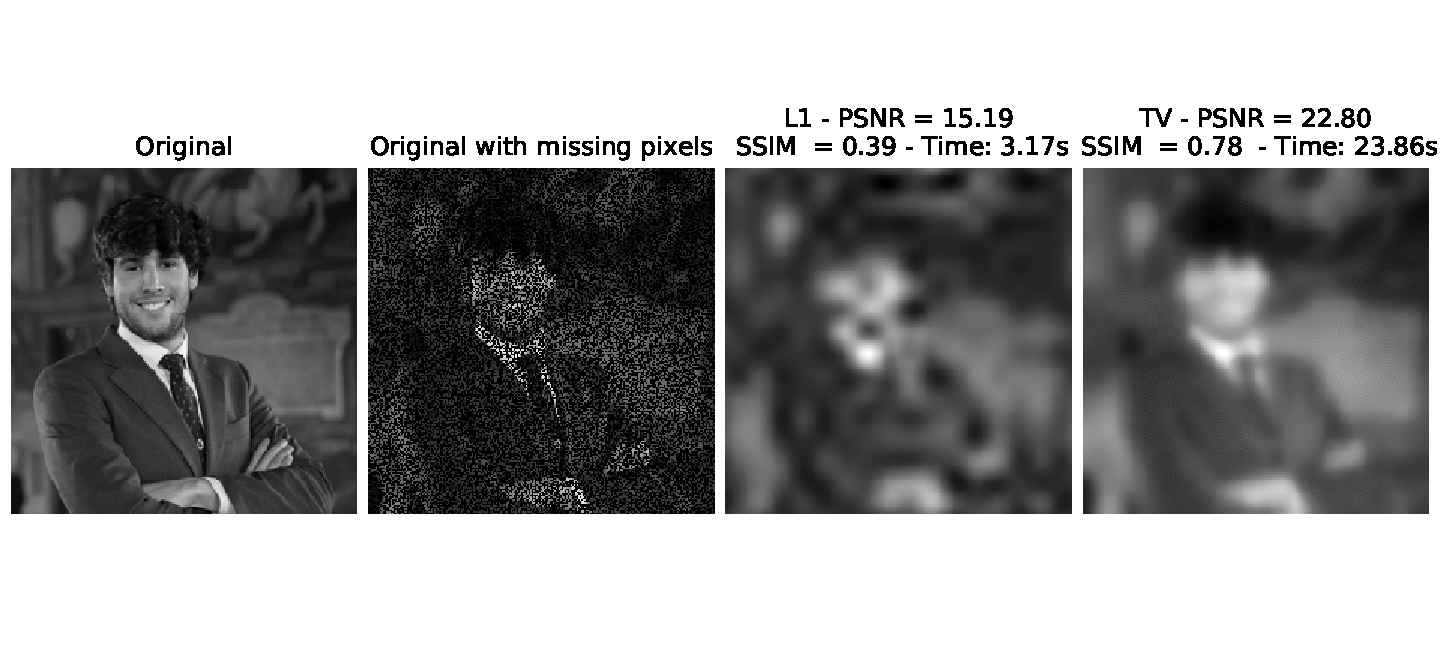
\includegraphics[width=17cm]{hw3/codes/exercise2/results/lambda_search/me_1.pdf}
    \caption{Results obtained with $\lambda = 1$}
    \label{fig:lambda-search-1}
\end{figure}

\begin{figure}
    \centering
    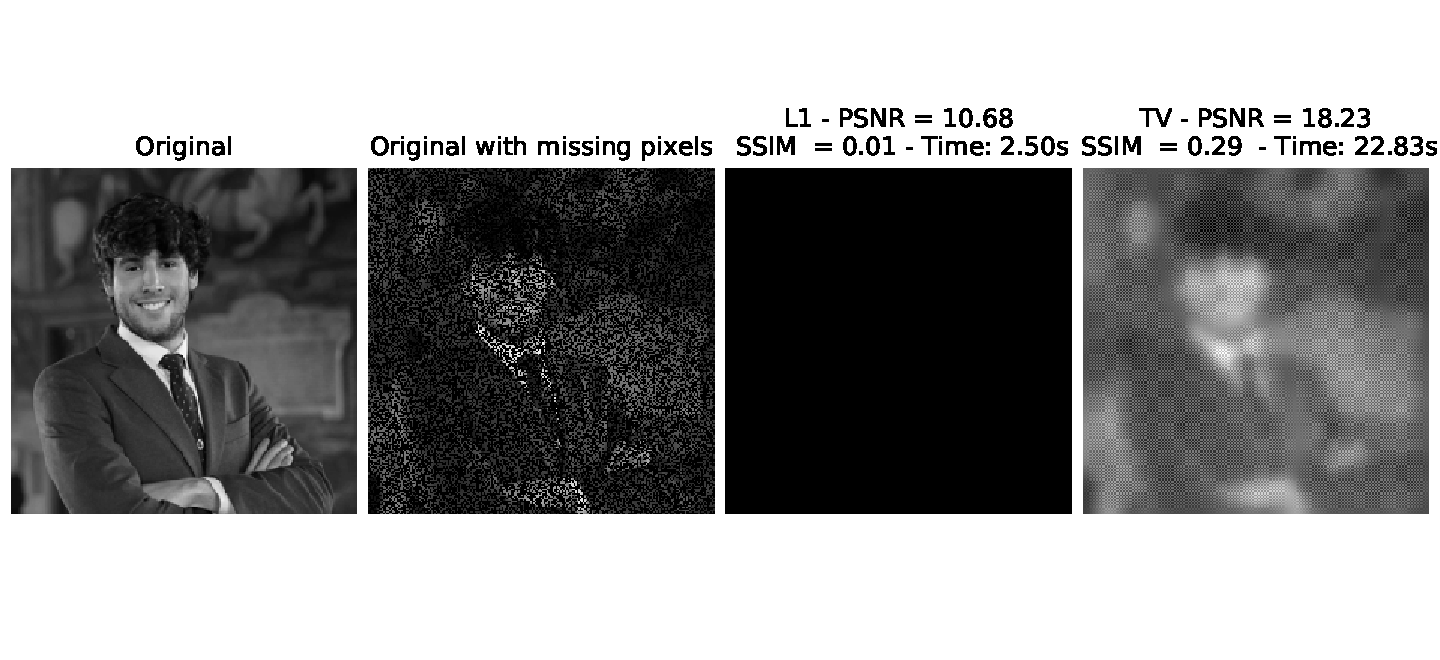
\includegraphics[width=17cm]{hw3/codes/exercise2/results/lambda_search/me_10.pdf}
    \caption{Results obtained with $\lambda = 10$}
    \label{fig:lambda-search-10}
\end{figure}

\begin{figure}
    \centering
    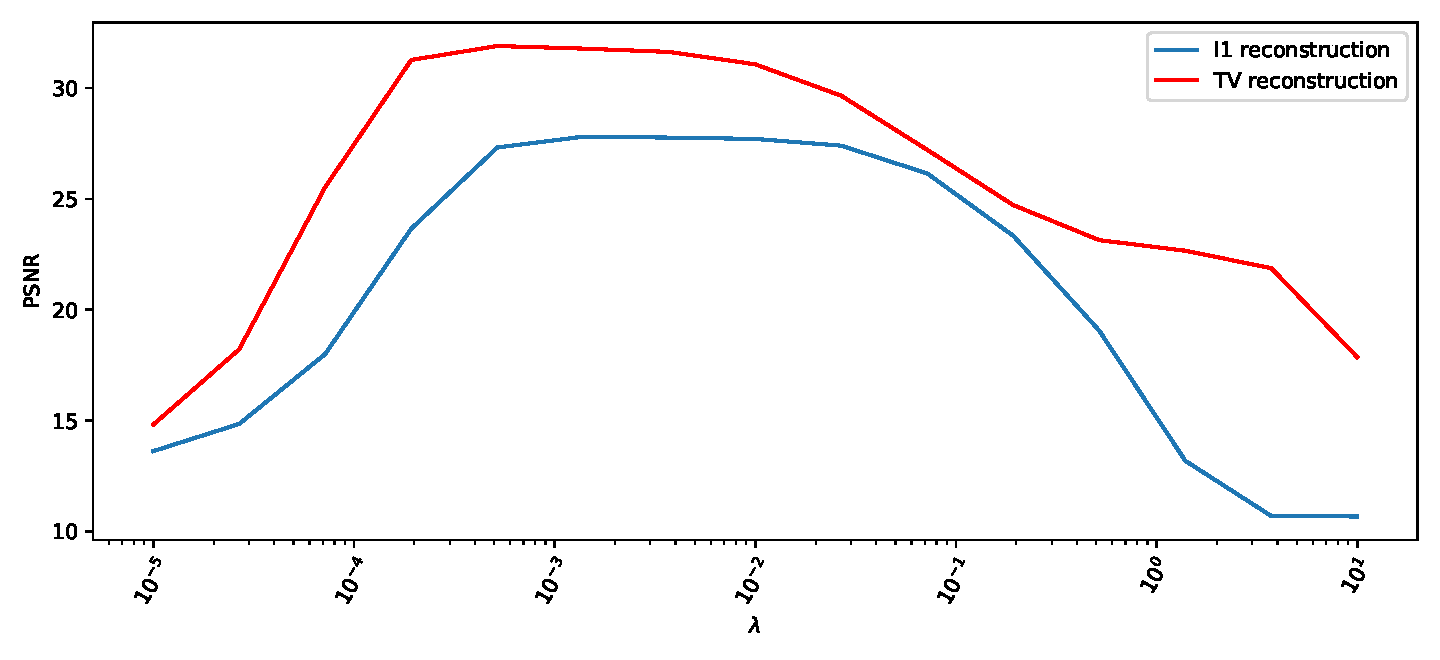
\includegraphics[width=14cm]{hw3/codes/exercise2/results/lambda_search/lambda_search.pdf}
    \caption{PSNR as a function of the regularization parameter $\lambda$}
    \label{fig:lambda-search}
\end{figure}

\subsection{Proximal methods convergence}

\begin{figure}
    \centering
    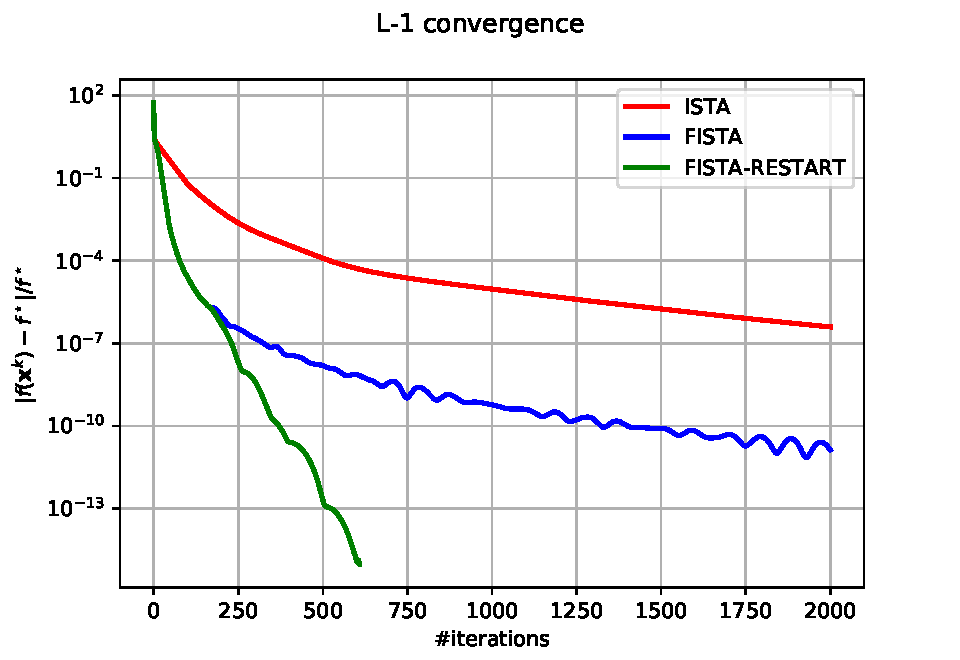
\includegraphics[width=10cm]{hw3/codes/exercise2/results/f_star_convergence.pdf}
    \caption{Convergence of ISTA, FISTA and FISTA Restart with respect to $F^\star$}
    \label{fig:f-star-convergence}
\end{figure}

\begin{figure}
    \centering
    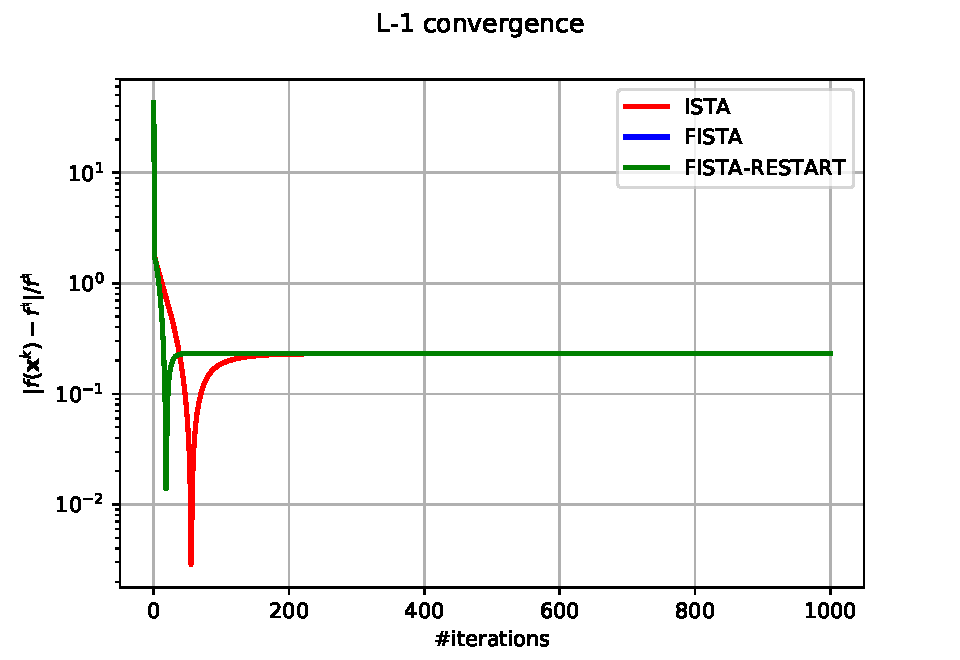
\includegraphics[width=10cm]{hw3/codes/exercise2/results/f_natural_convergence.pdf}
    \caption{Convergence of ISTA, FISTA and FISTA Restart with respect to $F^\natural$}
    \label{fig:f-natural-convergence}
\end{figure}

\subsection{Wavelet in-painting and NN unrolling comparison}
\subsubsection{500 iterations}
\begin{figure}
    \centering
    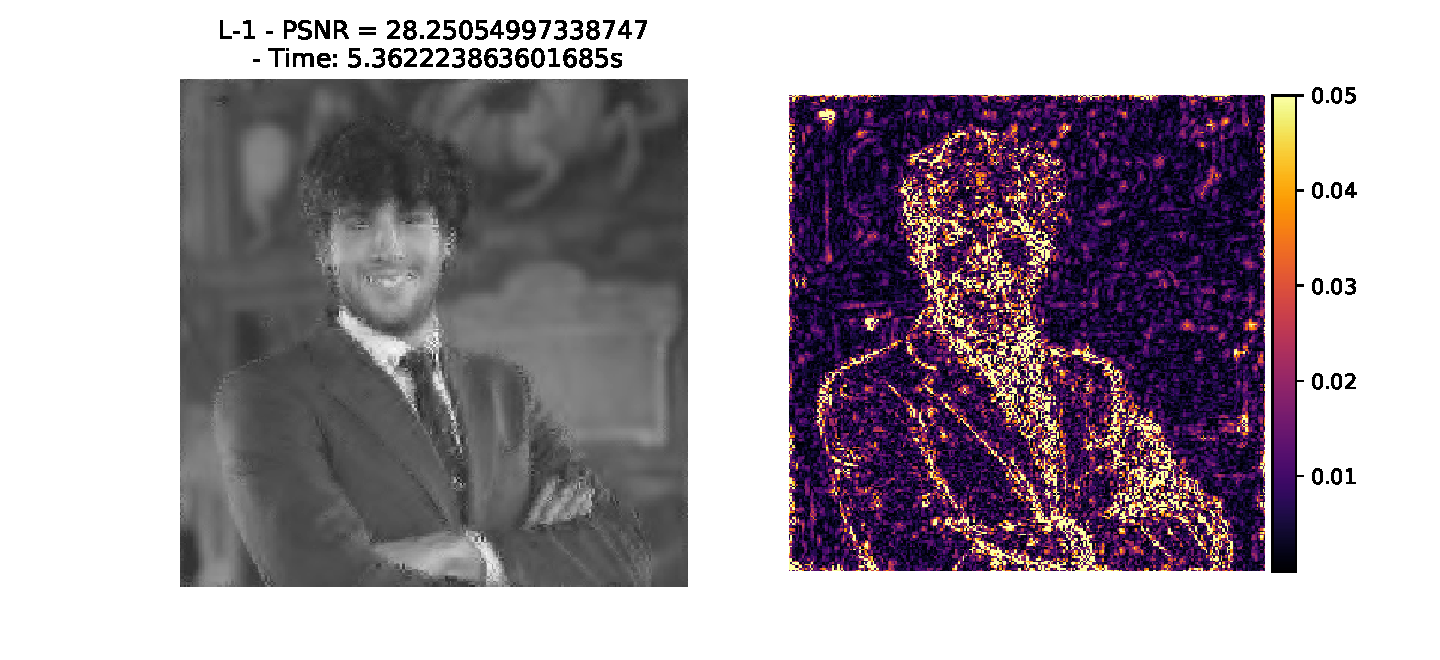
\includegraphics[width=12cm]{hw3/codes/exercise2/results/comparisons/me_comparison_l1_500.pdf}
    \caption{Results with 500 iterations and $\ell$-1 norm regularizer, with error mask on the left}
    \label{fig:comparison-l1-500}
\end{figure}

\begin{figure}
    \centering
    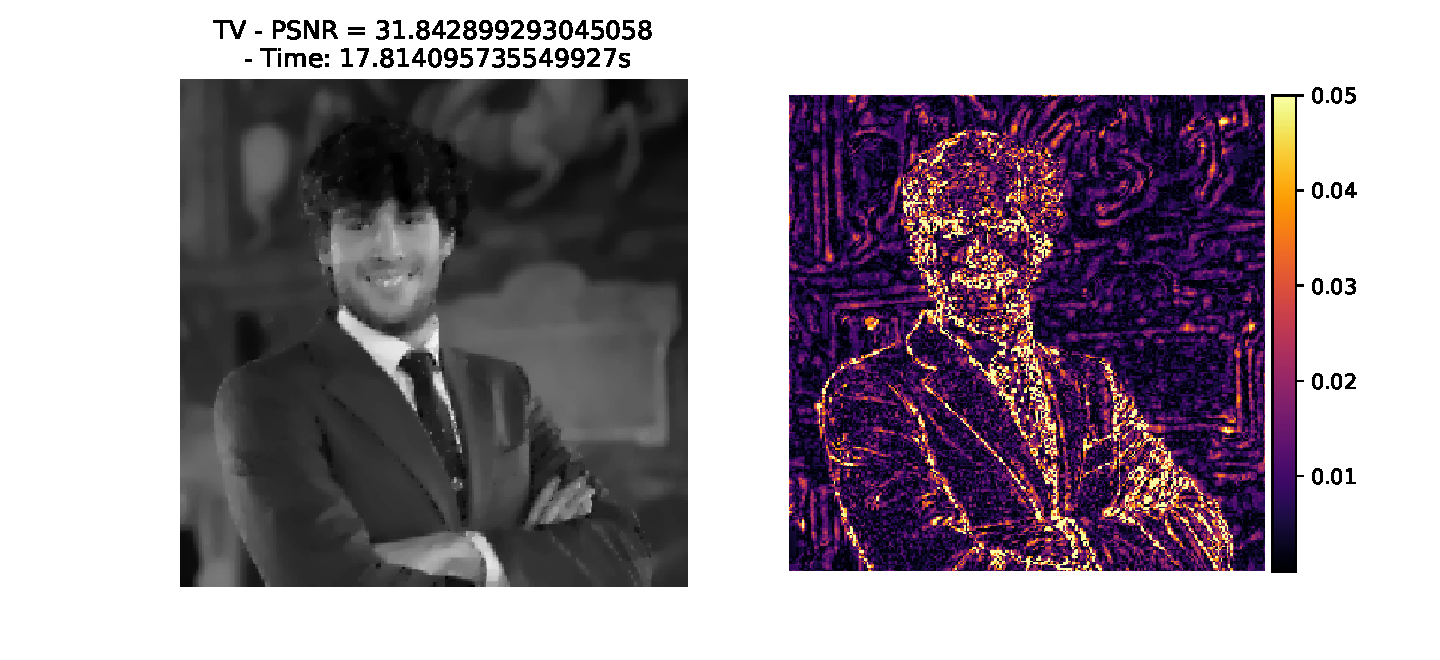
\includegraphics[width=12cm]{hw3/codes/exercise2/results/comparisons/me_comparison_tv_500.pdf}
    \caption{Results with 500 iterations and TV-norm regularizer, with error mask on the left}
    \label{fig:comparison-tv-500}
\end{figure}

\begin{figure}
    \centering
    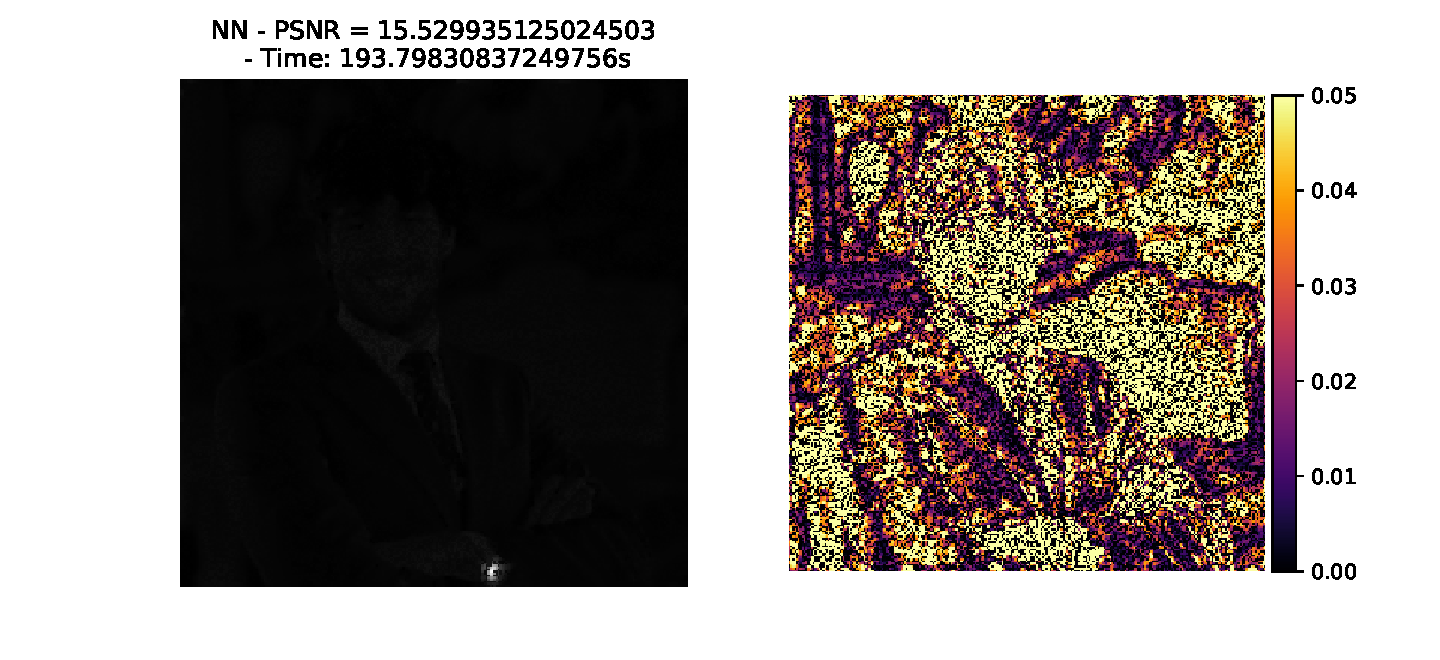
\includegraphics[width=12cm]{hw3/codes/exercise2/results/comparisons/me_comparison_nn_500.pdf}
    \caption{Results with 500 iterations and unrolled NN, with error mask on the left}
    \label{fig:comparison-nn-500}
\end{figure}

\subsubsection{5 iterations}
\begin{figure}
    \centering
    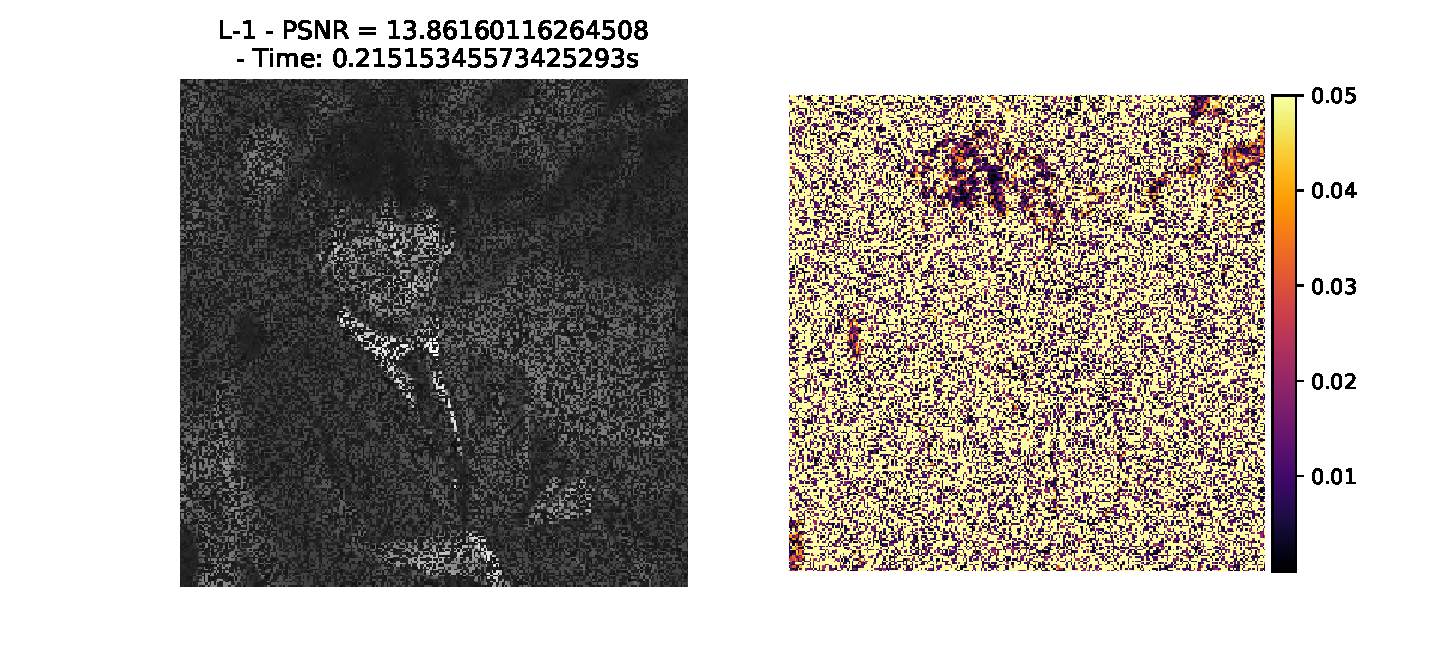
\includegraphics[width=12cm]{hw3/codes/exercise2/results/comparisons/me_comparison_l1_5.pdf}
    \caption{Results with 5 iterations and $\ell$-1 norm regularizer, with error mask on the left}
    \label{fig:comparison-l1-5}
\end{figure}

\begin{figure}
    \centering
    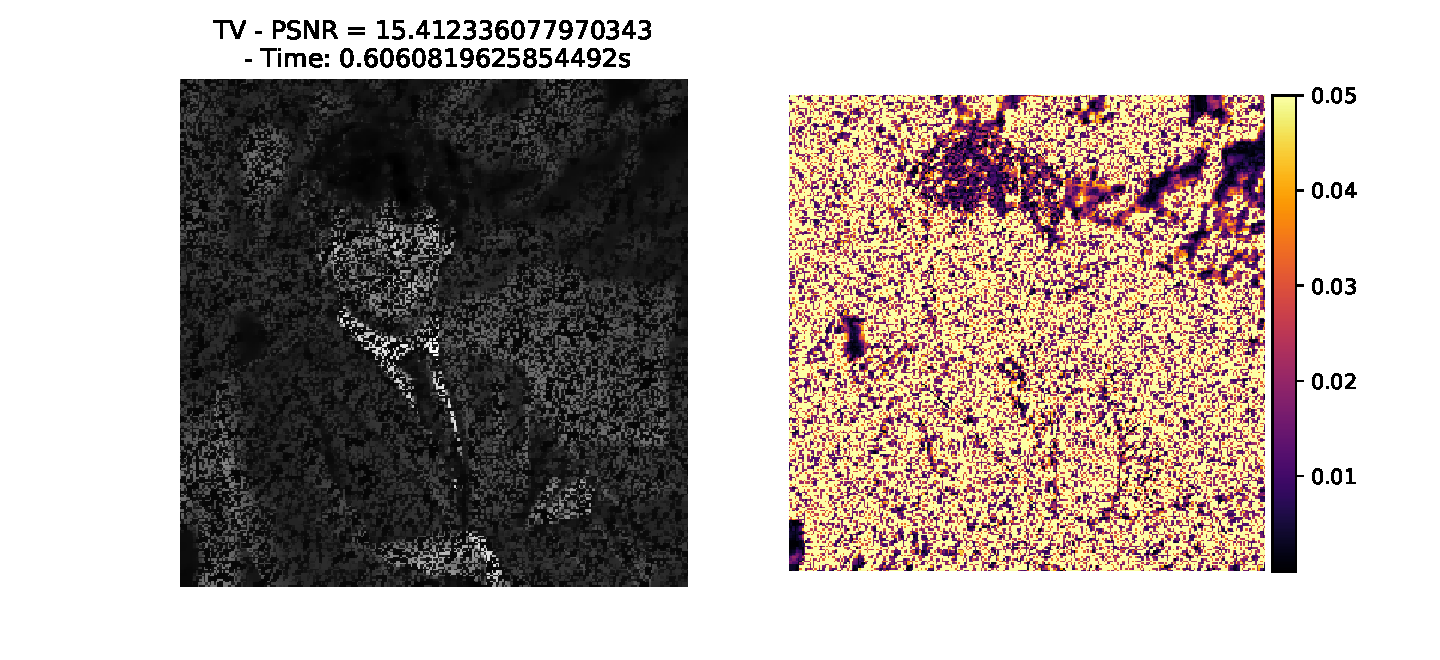
\includegraphics[width=12cm]{hw3/codes/exercise2/results/comparisons/me_comparison_tv_5.pdf}
    \caption{Results with 5 iterations and TV-norm regularizer, with error mask on the left}
    \label{fig:comparison-tv-5}
\end{figure}

\begin{figure}
    \centering
    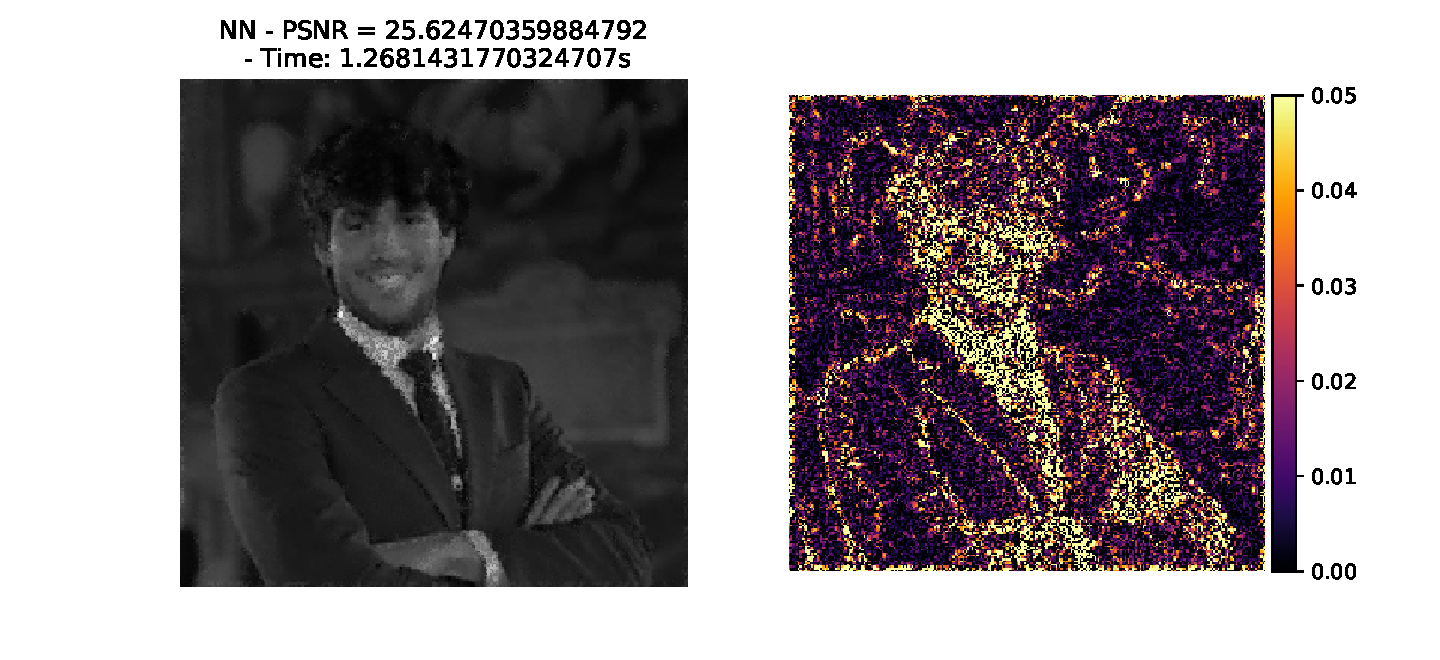
\includegraphics[width=12cm]{hw3/codes/exercise2/results/comparisons/me_comparison_nn_5.pdf}
    \caption{Results with 5 iterations and unrolled NN, with error mask on the left}
    \label{fig:comparison-nn-5}
\end{figure}

\end{document}